\section{The First Machine: A Traffic Light Controller}
\label{tutorial_03}

% a first machine, e.g. a traffic light with booleans for signals.  We introduce guards, resulting in the proof obligations to be discharged automatically. We explain how proof lables are read, without changing to the proof perspective.

\tick{\textbf{Goals:} The objective of this section is to get acquainted with the modeling environment. We will create a very simple model consisting of just one file to develop a feel for Rodin and Event-B.}

In this tutorial, we will create a model of a traffic light controller.  We will use this example in repeatedly in subsequent Sections.  The following image depicts what we are trying to achieve:

\begin{center}
	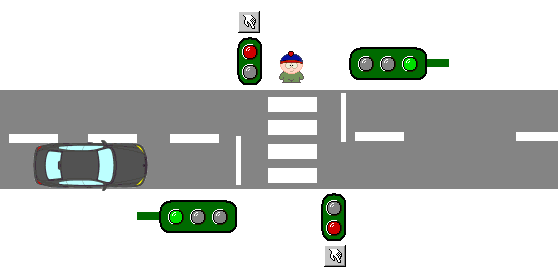
\includegraphics[width=0.7\textwidth]{img/tutorial/trafficlight.png}
\end{center}

In this Section, we will implement a simplified controller with the following differences:
\begin{itemize}
	\item We model the signals with booleans to indicated ``stop'' (false) and ``go'' (true).  We do not model colors (yet).
	\item We do not model the push button yet.
\end{itemize}

\subsection{Project Setup}

Models typically consist of multiple files that are managed in a Project (\ref{project}).  Create a new Event-B Project \textsf{File $\rangle$ New $\rangle$ Event-B Project}.  Give the project the name \texttt{tutorial-03}.

\warning{Eclipse supports different types of Projects.  The Project must have the Rodin Nature (\ref{rodin_nature}) to work.  A project can have more than one nature.}

Next, create a new Event-B Component (\ref{eventb_component}).  Either use \textsf{File $\rangle$ New $\rangle$ Event-B Component}, or right-click on the newly created project and select \textsf{New $\rangle$ Event-B Component}.  Use \texttt{mac} as the component name and click \textsf{Finish}.  This will create a Machine (\ref{machine}) file.

The newly created Component will open in the structural editor (\ref{structural_editor}).  The editor has four tabs at the bottom.  The \textsf{Pretty Print} shows the model as a whole with color highlighting, but it cannot be edited here.  This is useful to inspect the model.  The \textsf{Edit} allows editing of the model.  It shows the six main sections of a machine (REFINES, SEES, etc.) in a collapsed state.  You can click on the little triangle to the left of a section to expand it.

The editor is \textit{form-based}.  This means that in well-defined places an appropriate control (text field, dropdown, etc.) allows modifications.

\info{Alternative editors are available as plug-ins.  The form editor has the advantage of guiding the user through the model, but it takes up a lot of real estate and can be slow on big models.  The text- based Camille Editor (\ref{camille}) is very popular.  Please visit the Rodin Wiki (\ref{rodin_wiki}) for the latest information.}


\subsection{Building the Model}

Back to the problem: Our objective is to build a simplified traffic light controller, as described in \ref{tutorial_3}.  We start with the model state.  We will model two traffic lights.  Therefore, we will create two variables, called \texttt{cars\_go} and \texttt{peds\_go}.  Go to the \textsf{Edit} tab in the editor and expand the \textsf{VARIABLES} section.  Click on the green plus-sign to create a new variable.

\subsubsection{Creating Variables}

You will see two fields, the left one prepopulated with \texttt{var1}.  Change this to \texttt{cars\_go}.  The second field (after the double-slash ``//'') is a comment field that can take any text.

\info{\textbf{Comments:} The comment field supports line breaks.  Note that it is not possible to ``comment out'' parts of the model, as you would expect in programming languages.  You can use the comment field to ``park'' predicates and other strings temporarily.}

Create the second variable (\texttt{peds\_go}) correspondingly.  Your editor should now look as follows:

TODO: Screenshot

Upon saving, the variables will be highlighted in red, indicating a problem.  The \textsf{Rodin Problems} View (\ref{rodin_problems_view}) shows corresponding error messages, in this case ``Variable cars\_go does not have a type''.

Types are provided by invariants.  Corresponding the the steps above, expand the \textsf{INVARIANTS} section and add two elements.  Invariants have labels (\ref{label}).  Default labels are generated (\texttt{inv1} and \texttt{inv2}).  The actual invariant is prepopulated with $\btrue$, representing logical true.  Change this to $cars\_go \in  BOOL$.  Event-B provides the build-in datatype \texttt{BOOL}, amongst others (\ref{datatypes}).

\info{\textbf{Mathematical Symbols:} Every mathematical symbol has an ASCII-representation that is substituted automatically.  To generate ``element of'' ($\in$), simply type a colon (``:'').  The editor will perform the substitution after a short delay.  The symbol view shows all supported mathematical symbols.  The symbol view discloses the ASCII representation by hovering over the symbol in question.}

After saving, you should see that the \textsf{EVENTS} section is highlighted in yellow.  Again, the \textsf{Rodin Problems} View gives us the reason: ``Variable cars\_go is not initialized''.  Every variable must be initialized in a way that is consistent with the model.

To fix this problem, expand the \textsf{EVENTS} and in turn the INITIALIZATION event (\ref{initialization}).  Add two elements in the \textsf{THEN} block.  These are actions that also have labels.  In the action fields, provide $cars\_go :=  FALSE$ and $peds\_go :=  FALSE$.

\subsubsection{State Transitions with Events}

Our traffic light controller cannot yet change its state.  To make this possible, we provide events (\ref{event}). We start with the traffic light for the pedestrians, and we will provide two events, one to set it to ``go'' and one to set it to ``stop''.

\warning{From now on, we won't describe the individual steps in the editor any more.  Instead, we will simply show the resulting model.} 

The two events will look as follows:

\pencil{
\begin{description}
	\EVT {set\_peds\_go}
		\begin{description}
		\BeginAct
			\begin{description}
			\nItemX{ act1 }{ peds\_go :=  TRUE }
			\end{description}
		\EndAct
		\end{description}
	\EVT {set\_peds\_stop}
		\begin{description}
		\BeginAct
			\begin{description}
			\nItemX{ act1 }{ peds\_go :=  FALSE }
			\end{description}
		\EndAct
		\end{description}
\end{description}
}

\subsubsection{Event parameters}

For the traffic light for the cars, we will present a different approach and use only one event with a parameter.  The event will use the new traffic light state as the argument.  The parameter is declared in the \textsf{any} section and typed in the \textsf{where} section:

\pencil{
\begin{description}
	\EVT {set\_cars}
		\begin{description}
		\AnyPrm
			\begin{description}
			\ItemX{ new\_value }
			\end{description}
		\WhereGrd
			\begin{description}
			\nItemX{ grd1 }{ new\_value \in  BOOL }
			\end{description}
		\ThenAct
			\begin{description}
			\nItemX{ act1 }{ cars\_go :=  new\_value }
			\end{description}
		\EndAct
		\end{description}
\end{description}
}

Note how the parameter is used in the action block.

\subsubsection{Invariants}

If this model would control a traffic light, we would have a problem, as nothing is preventing the model from setting both traffic lights to \texttt{TRUE}.  The reason is that so far we only modeled the domain (the traffic lights and their states), and not the requirements.  We have the following safety requirement:

\begin{center}REQ-1: Both traffic lights must not be \texttt{TRUE} at the same time.\end{center}

We can model this requirement with the following invariant (please add this invariant to the model):
\[
\lnot  (cars\_go = TRUE \land  peds\_go = TRUE)
\]

Obviously, this invariant can be violated, and Rodin can tell us that.  The Explorer (\ref{eventb_explorer}) provides this information in various ways.  Go to the explorer and expand the project (\texttt{tutorial-03}), the machine (\texttt{mac}) and the entry ``Proof Obligations''.  You should see four proof obligations, two of which are not discharged.

\info{Make sure that you understand the proof obligation labels (\ref{po_labels}).  Also, the proof obligations can also be found via other entries.  Elements that have non-discharged proof obligations as children are marked with a small question mark.  For instance, \texttt{inv3} has all proof obligations as children, while the event \texttt{set\_cars} has one.}

To prevent the invariant from being violated (and therefore to allow all proof obligations to be discharged), we need to strengthen the guards (\ref{guard}) of the events.

\warning{Before looking at the solution, try to fix the model yourself.}

This concludes the tutorial.

\subsection{The Final Traffic Light Model}

\pencil{
\begin{description}
\MACHINE{mac}
\VARIABLES
	\begin{description}
		\Item{ cars\_go }
		\Item{ peds\_go }
	\end{description}
\INVARIANTS
	\begin{description}
		\nItemX{ inv1 }{ cars\_go \in  BOOL }
		\nItemX{ inv2 }{ peds\_go \in  BOOL }
		\nItemX{ inv3 }{ \lnot  (cars\_go = TRUE \land  peds\_go = TRUE) }
	\end{description}
\EVENTS
	\INITIALISATION
		\begin{description}
		\BeginAct
			\begin{description}
			\nItemX{ act1 }{ cars\_go :=  FALSE }
			\nItemX{ act2 }{ peds\_go :=  FALSE }
			\end{description}
		\EndAct
		\end{description}
	\EVT {set\_peds\_go}
		\begin{description}
		\WhenGrd
			\begin{description}
			\nItemX{ grd1 }{ cars\_go = FALSE }
			\end{description}
		\ThenAct
			\begin{description}
			\nItemX{ act1 }{ peds\_go :=  TRUE }
			\end{description}
		\EndAct
		\end{description}
	\EVT {set\_peds\_stop}
		\begin{description}
		\BeginAct
			\begin{description}
			\nItemX{ act1 }{ peds\_go :=  FALSE }
			\end{description}
		\EndAct
		\end{description}
	\EVT {set\_cars}
		\begin{description}
		\AnyPrm
			\begin{description}
			\ItemX{ new\_value }
			\end{description}
		\WhereGrd
			\begin{description}
			\nItemX{ grd1 }{ new\_value \in  BOOL }
			\nItemX{ grd2 }{ new\_value = TRUE \limp  peds\_go = FALSE }
			\end{description}
		\ThenAct
			\begin{description}
			\nItemX{ act1 }{ cars\_go :=  new\_value }
			\end{description}
		\EndAct
		\end{description}
\END
\end{description}
}

